\chapter{Especificação do Sistema}

\section{Hardware - Arduino Uno R3}
\begin{figure}[H]
    \centering
    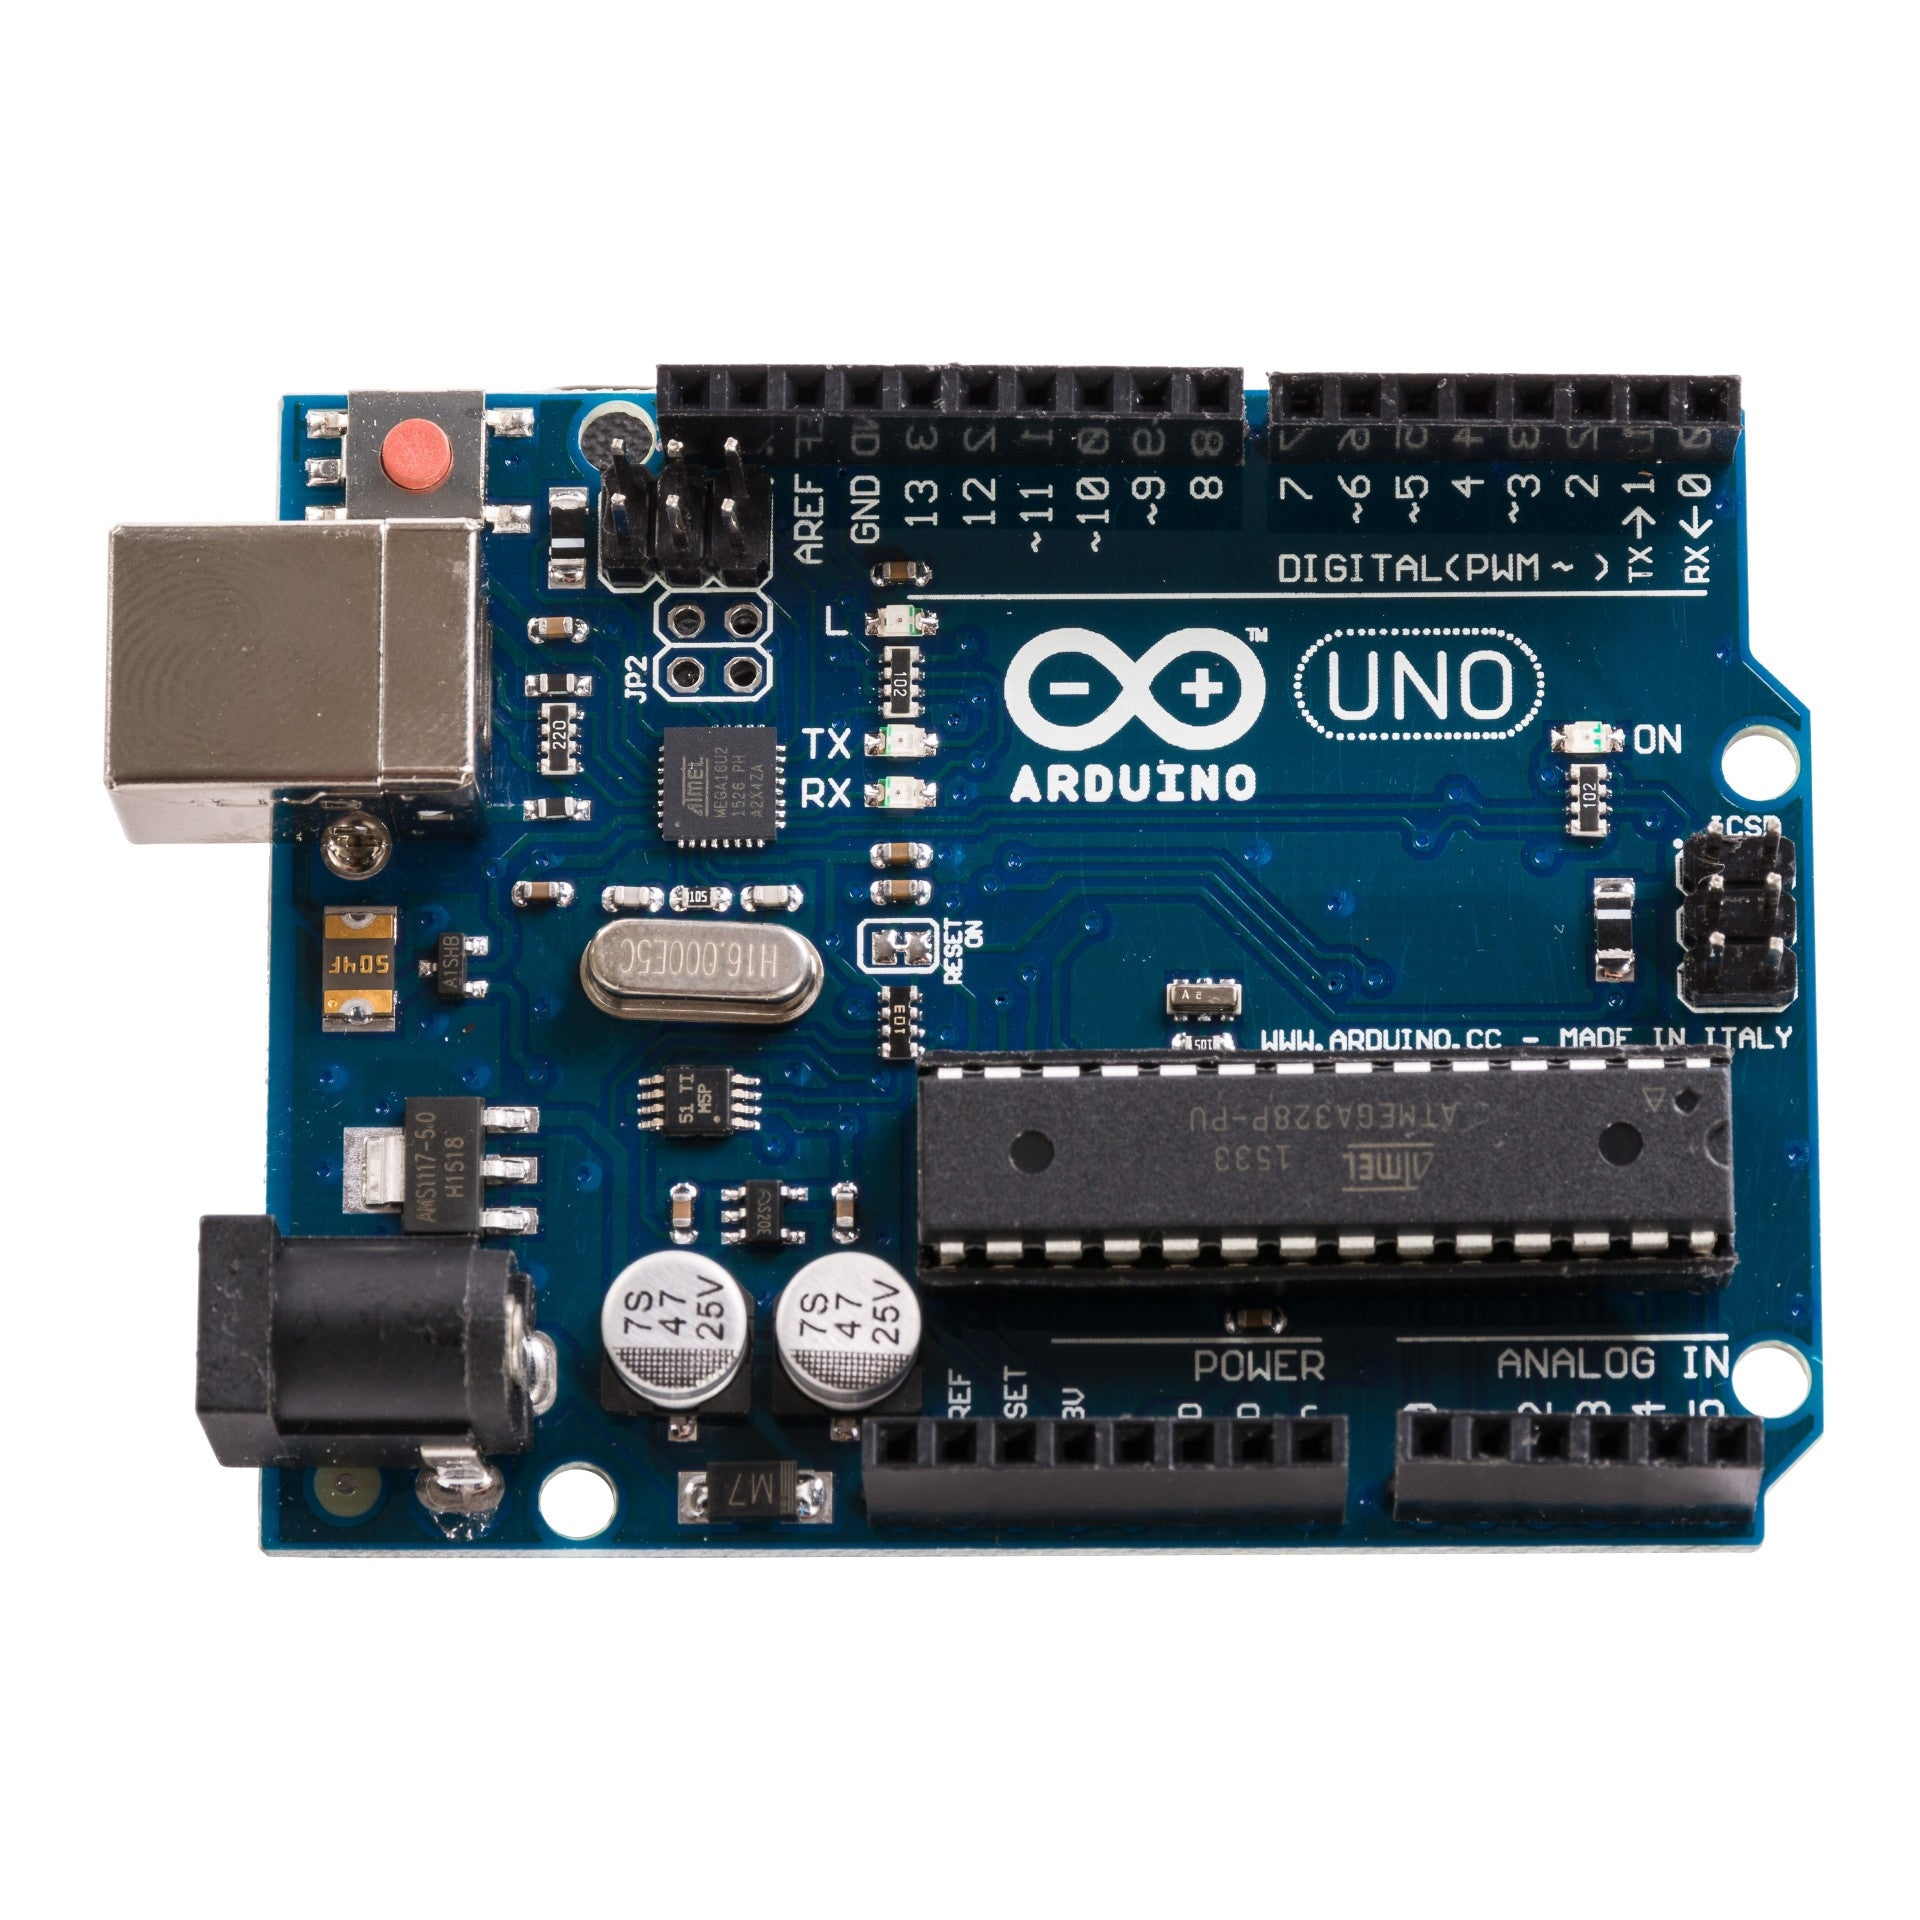
\includegraphics[scale=0.15]{images/Arduino_Board.jpg}
    \selectlanguage{portuguese}\caption{Arduino Uno R3}
\end{figure}
O design da PCB do Arduino Uno utiliza componentes SMD\footnote{Surface Mount Device}.

O micro-controlador inserido nesta placa é o \textbf{ATmega328} - MCU\footnote{Micro Controller Unit} da família AVR\footnote{Alf and Vegard's RISC} e Arquitetura Harvard (armazena o programa e as variáveis em unidades diferentes.). É um dispositivo de 8-bits, isto é, a sua arquitetura é capaz de gerir 8 sinais em paralelo.

Este chip tem 3 tipos de memória:
\begin{itemize}
    \item \textbf{Flash}: 32kB. Utilizada para armazenar o código compilado da aplicação, dado ser memória \textbf{Não Volátil}.
    \item \textbf{SRAM}: 2kB. Armazenamento de variáveis. \textbf{Volátil}.
    \item \textbf{EEPROM}: 1kB. Armazenamento de dados, que necessitam persistência. \textbf{Não Volátil}.
\end{itemize}

Para armazenamento do código compilado, dado que a MCU não é capaz de comunicar diretamente por USB, precisa de uma `ponte' que converta os sinais do host USB para a interface UART\footnote{Universal Asynchronous Receiver-Transmiter} - o \textbf{ATmega16U2}.

\begin{figure}[H]
    \centering
    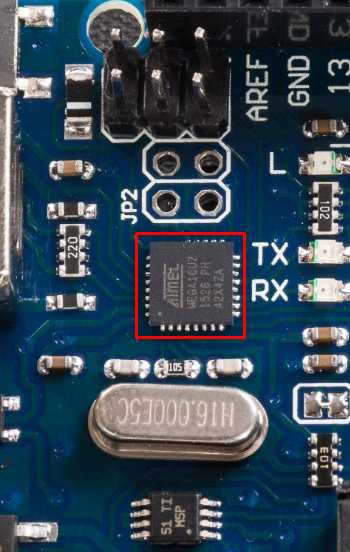
\includegraphics[scale=0.8, angle=-90]{images/atmega16u2.png}
    \selectlanguage{portuguese}\caption{ATmega16U2}
\end{figure}

\section{Software - C/C++}

Para facilidade de uso pelos consumidores o \textit{chipset} (ATmega328) é previamente programado com um \textit{\textbf{bootloader}}. Este é basicamente o controlador do processo de `arranque' da placa Arduino.

Dado que o código é desenvolvido numa arquitetura diferente da arquitetura destino (x86\_x64 para Arm), o código é compilado em \textit{cross-compiling} e denominado de \textit{\textbf{firmware}}. É carregado via USB como discutido anteriormente e apenas uma vez, dada a persistência da memória. 
\newpage
Exemplo de \textit{cross-compiling} de programa(em ambiente Linux baseado em Debian/Ubuntu).

\begin{lstlisting}[language=bash]
// Install packages
sudo apt-get install gcc-arm-linux-gnueabi 
g++-arm-linux-gnueabi

// Compile
arm-linux-gnueabi-gcc helloworld.c -o helloworld-arm 
-static
// Run
./helloworld-arm
// Read Architecture
readelf -h helloworld-arm
\end{lstlisting}